% Created by tikzDevice version 0.12.3.1 on 2022-08-17 16:47:27
% !TEX encoding = UTF-8 Unicode
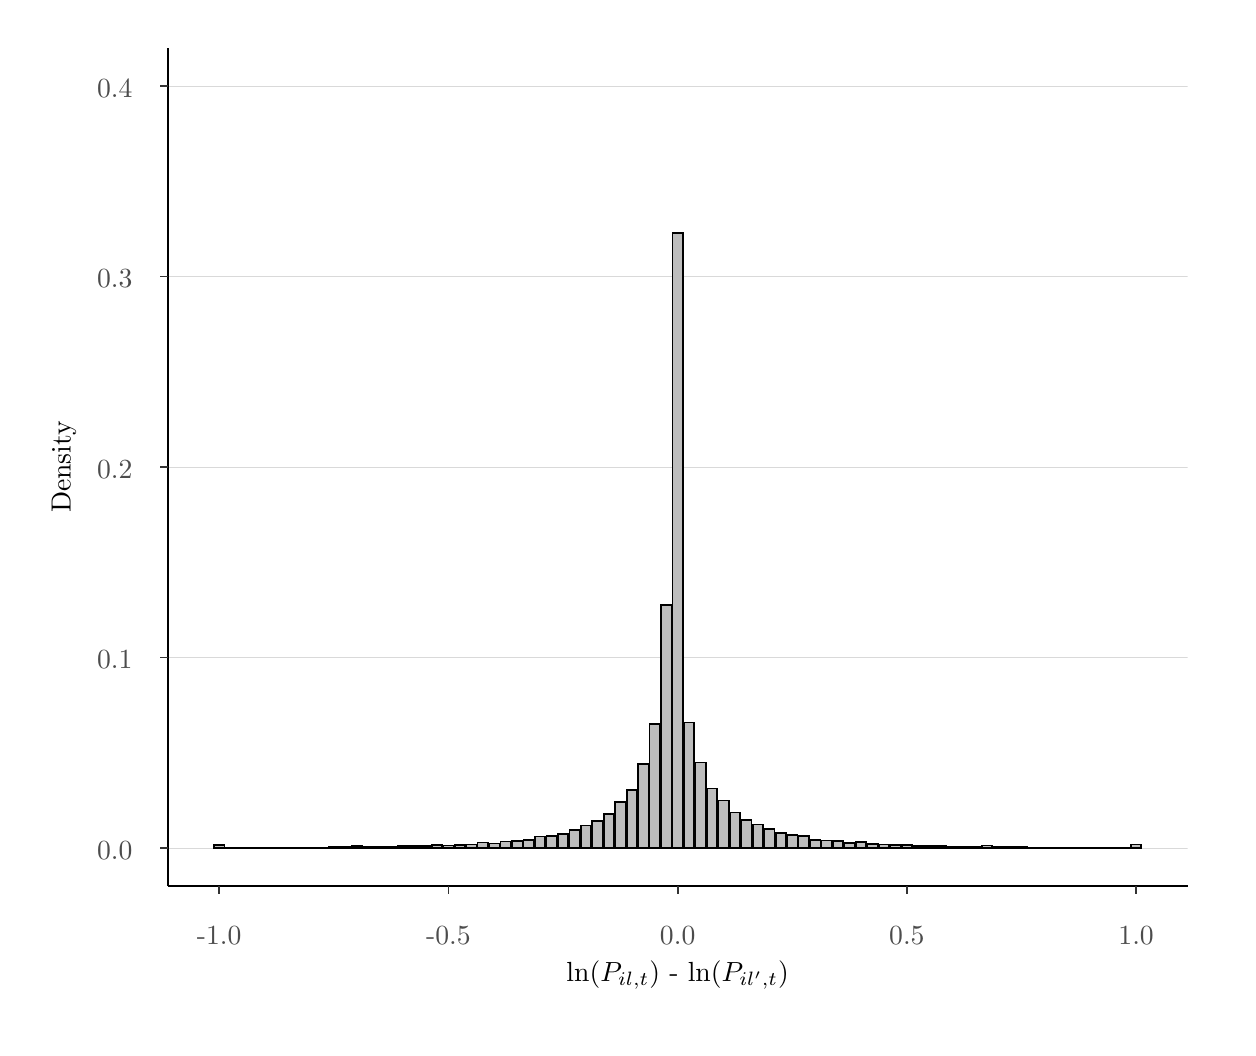
\begin{tikzpicture}[x=1pt,y=1pt]
\definecolor{fillColor}{RGB}{255,255,255}
\path[use as bounding box,fill=fillColor,fill opacity=0.00] (0,0) rectangle (433.62,361.35);
\begin{scope}
\path[clip] (  0.00,  0.00) rectangle (433.62,361.35);
\definecolor{drawColor}{RGB}{255,255,255}
\definecolor{fillColor}{RGB}{255,255,255}

\path[draw=drawColor,line width= 0.6pt,line join=round,line cap=round,fill=fillColor] (  0.00,  0.00) rectangle (433.62,361.35);
\end{scope}
\begin{scope}
\path[clip] ( 50.59, 51.15) rectangle (419.17,354.12);
\definecolor{drawColor}{RGB}{255,255,255}

\path[draw=drawColor,line width= 0.3pt,line join=round] ( 50.59, 99.35) --
	(419.17, 99.35);

\path[draw=drawColor,line width= 0.3pt,line join=round] ( 50.59,168.21) --
	(419.17,168.21);

\path[draw=drawColor,line width= 0.3pt,line join=round] ( 50.59,237.07) --
	(419.17,237.07);

\path[draw=drawColor,line width= 0.3pt,line join=round] ( 50.59,305.92) --
	(419.17,305.92);

\path[draw=drawColor,line width= 0.3pt,line join=round] (110.63, 51.15) --
	(110.63,354.12);

\path[draw=drawColor,line width= 0.3pt,line join=round] (193.46, 51.15) --
	(193.46,354.12);

\path[draw=drawColor,line width= 0.3pt,line join=round] (276.30, 51.15) --
	(276.30,354.12);

\path[draw=drawColor,line width= 0.3pt,line join=round] (359.13, 51.15) --
	(359.13,354.12);
\definecolor{drawColor}{gray}{0.85}

\path[draw=drawColor,line width= 0.1pt,line join=round] ( 50.59, 64.92) --
	(419.17, 64.92);

\path[draw=drawColor,line width= 0.1pt,line join=round] ( 50.59,133.78) --
	(419.17,133.78);

\path[draw=drawColor,line width= 0.1pt,line join=round] ( 50.59,202.64) --
	(419.17,202.64);

\path[draw=drawColor,line width= 0.1pt,line join=round] ( 50.59,271.49) --
	(419.17,271.49);

\path[draw=drawColor,line width= 0.1pt,line join=round] ( 50.59,340.35) --
	(419.17,340.35);
\definecolor{drawColor}{RGB}{0,0,0}
\definecolor{fillColor}{gray}{0.74}

\path[draw=drawColor,line width= 0.6pt,line cap=rect,fill=fillColor] ( 67.34, 64.92) rectangle ( 71.07, 66.12);

\path[draw=drawColor,line width= 0.6pt,line cap=rect,fill=fillColor] ( 71.49, 64.92) rectangle ( 75.21, 65.01);

\path[draw=drawColor,line width= 0.6pt,line cap=rect,fill=fillColor] ( 75.63, 64.92) rectangle ( 79.36, 65.03);

\path[draw=drawColor,line width= 0.6pt,line cap=rect,fill=fillColor] ( 79.77, 64.92) rectangle ( 83.50, 65.05);

\path[draw=drawColor,line width= 0.6pt,line cap=rect,fill=fillColor] ( 83.91, 64.92) rectangle ( 87.64, 65.04);

\path[draw=drawColor,line width= 0.6pt,line cap=rect,fill=fillColor] ( 88.05, 64.92) rectangle ( 91.78, 65.06);

\path[draw=drawColor,line width= 0.6pt,line cap=rect,fill=fillColor] ( 92.19, 64.92) rectangle ( 95.92, 65.08);

\path[draw=drawColor,line width= 0.6pt,line cap=rect,fill=fillColor] ( 96.34, 64.92) rectangle (100.06, 65.10);

\path[draw=drawColor,line width= 0.6pt,line cap=rect,fill=fillColor] (100.48, 64.92) rectangle (104.21, 65.12);

\path[draw=drawColor,line width= 0.6pt,line cap=rect,fill=fillColor] (104.62, 64.92) rectangle (108.35, 65.15);

\path[draw=drawColor,line width= 0.6pt,line cap=rect,fill=fillColor] (108.76, 64.92) rectangle (112.49, 65.17);

\path[draw=drawColor,line width= 0.6pt,line cap=rect,fill=fillColor] (112.90, 64.92) rectangle (116.63, 65.30);

\path[draw=drawColor,line width= 0.6pt,line cap=rect,fill=fillColor] (117.05, 64.92) rectangle (120.77, 65.76);

\path[draw=drawColor,line width= 0.6pt,line cap=rect,fill=fillColor] (121.19, 64.92) rectangle (124.91, 65.30);

\path[draw=drawColor,line width= 0.6pt,line cap=rect,fill=fillColor] (125.33, 64.92) rectangle (129.06, 65.38);

\path[draw=drawColor,line width= 0.6pt,line cap=rect,fill=fillColor] (129.47, 64.92) rectangle (133.20, 65.37);

\path[draw=drawColor,line width= 0.6pt,line cap=rect,fill=fillColor] (133.61, 64.92) rectangle (137.34, 65.57);

\path[draw=drawColor,line width= 0.6pt,line cap=rect,fill=fillColor] (137.75, 64.92) rectangle (141.48, 65.55);

\path[draw=drawColor,line width= 0.6pt,line cap=rect,fill=fillColor] (141.90, 64.92) rectangle (145.62, 65.61);

\path[draw=drawColor,line width= 0.6pt,line cap=rect,fill=fillColor] (146.04, 64.92) rectangle (149.77, 65.92);

\path[draw=drawColor,line width= 0.6pt,line cap=rect,fill=fillColor] (150.18, 64.92) rectangle (153.91, 65.86);

\path[draw=drawColor,line width= 0.6pt,line cap=rect,fill=fillColor] (154.32, 64.92) rectangle (158.05, 66.03);

\path[draw=drawColor,line width= 0.6pt,line cap=rect,fill=fillColor] (158.46, 64.92) rectangle (162.19, 66.19);

\path[draw=drawColor,line width= 0.6pt,line cap=rect,fill=fillColor] (162.60, 64.92) rectangle (166.33, 66.89);

\path[draw=drawColor,line width= 0.6pt,line cap=rect,fill=fillColor] (166.75, 64.92) rectangle (170.47, 66.56);

\path[draw=drawColor,line width= 0.6pt,line cap=rect,fill=fillColor] (170.89, 64.92) rectangle (174.62, 67.29);

\path[draw=drawColor,line width= 0.6pt,line cap=rect,fill=fillColor] (175.03, 64.92) rectangle (178.76, 67.42);

\path[draw=drawColor,line width= 0.6pt,line cap=rect,fill=fillColor] (179.17, 64.92) rectangle (182.90, 67.71);

\path[draw=drawColor,line width= 0.6pt,line cap=rect,fill=fillColor] (183.31, 64.92) rectangle (187.04, 69.07);

\path[draw=drawColor,line width= 0.6pt,line cap=rect,fill=fillColor] (187.46, 64.92) rectangle (191.18, 69.31);

\path[draw=drawColor,line width= 0.6pt,line cap=rect,fill=fillColor] (191.60, 64.92) rectangle (195.32, 70.10);

\path[draw=drawColor,line width= 0.6pt,line cap=rect,fill=fillColor] (195.74, 64.92) rectangle (199.47, 71.45);

\path[draw=drawColor,line width= 0.6pt,line cap=rect,fill=fillColor] (199.88, 64.92) rectangle (203.61, 73.01);

\path[draw=drawColor,line width= 0.6pt,line cap=rect,fill=fillColor] (204.02, 64.92) rectangle (207.75, 74.67);

\path[draw=drawColor,line width= 0.6pt,line cap=rect,fill=fillColor] (208.16, 64.92) rectangle (211.89, 77.16);

\path[draw=drawColor,line width= 0.6pt,line cap=rect,fill=fillColor] (212.31, 64.92) rectangle (216.03, 81.45);

\path[draw=drawColor,line width= 0.6pt,line cap=rect,fill=fillColor] (216.45, 64.92) rectangle (220.18, 85.78);

\path[draw=drawColor,line width= 0.6pt,line cap=rect,fill=fillColor] (220.59, 64.92) rectangle (224.32, 95.16);

\path[draw=drawColor,line width= 0.6pt,line cap=rect,fill=fillColor] (224.73, 64.92) rectangle (228.46,109.76);

\path[draw=drawColor,line width= 0.6pt,line cap=rect,fill=fillColor] (228.87, 64.92) rectangle (232.60,152.81);

\path[draw=drawColor,line width= 0.6pt,line cap=rect,fill=fillColor] (233.01, 64.92) rectangle (236.74,287.25);

\path[draw=drawColor,line width= 0.6pt,line cap=rect,fill=fillColor] (237.16, 64.92) rectangle (240.88,110.26);

\path[draw=drawColor,line width= 0.6pt,line cap=rect,fill=fillColor] (241.30, 64.92) rectangle (245.03, 95.81);

\path[draw=drawColor,line width= 0.6pt,line cap=rect,fill=fillColor] (245.44, 64.92) rectangle (249.17, 86.45);

\path[draw=drawColor,line width= 0.6pt,line cap=rect,fill=fillColor] (249.58, 64.92) rectangle (253.31, 82.09);

\path[draw=drawColor,line width= 0.6pt,line cap=rect,fill=fillColor] (253.72, 64.92) rectangle (257.45, 77.78);

\path[draw=drawColor,line width= 0.6pt,line cap=rect,fill=fillColor] (257.87, 64.92) rectangle (261.59, 75.15);

\path[draw=drawColor,line width= 0.6pt,line cap=rect,fill=fillColor] (262.01, 64.92) rectangle (265.73, 73.40);

\path[draw=drawColor,line width= 0.6pt,line cap=rect,fill=fillColor] (266.15, 64.92) rectangle (269.88, 71.82);

\path[draw=drawColor,line width= 0.6pt,line cap=rect,fill=fillColor] (270.29, 64.92) rectangle (274.02, 70.42);

\path[draw=drawColor,line width= 0.6pt,line cap=rect,fill=fillColor] (274.43, 64.92) rectangle (278.16, 69.60);

\path[draw=drawColor,line width= 0.6pt,line cap=rect,fill=fillColor] (278.57, 64.92) rectangle (282.30, 69.33);

\path[draw=drawColor,line width= 0.6pt,line cap=rect,fill=fillColor] (282.72, 64.92) rectangle (286.44, 67.92);

\path[draw=drawColor,line width= 0.6pt,line cap=rect,fill=fillColor] (286.86, 64.92) rectangle (290.59, 67.62);

\path[draw=drawColor,line width= 0.6pt,line cap=rect,fill=fillColor] (291.00, 64.92) rectangle (294.73, 67.45);

\path[draw=drawColor,line width= 0.6pt,line cap=rect,fill=fillColor] (295.14, 64.92) rectangle (298.87, 66.74);

\path[draw=drawColor,line width= 0.6pt,line cap=rect,fill=fillColor] (299.28, 64.92) rectangle (303.01, 67.03);

\path[draw=drawColor,line width= 0.6pt,line cap=rect,fill=fillColor] (303.42, 64.92) rectangle (307.15, 66.32);

\path[draw=drawColor,line width= 0.6pt,line cap=rect,fill=fillColor] (307.57, 64.92) rectangle (311.29, 66.15);

\path[draw=drawColor,line width= 0.6pt,line cap=rect,fill=fillColor] (311.71, 64.92) rectangle (315.44, 65.93);

\path[draw=drawColor,line width= 0.6pt,line cap=rect,fill=fillColor] (315.85, 64.92) rectangle (319.58, 66.01);

\path[draw=drawColor,line width= 0.6pt,line cap=rect,fill=fillColor] (319.99, 64.92) rectangle (323.72, 65.70);

\path[draw=drawColor,line width= 0.6pt,line cap=rect,fill=fillColor] (324.13, 64.92) rectangle (327.86, 65.63);

\path[draw=drawColor,line width= 0.6pt,line cap=rect,fill=fillColor] (328.28, 64.92) rectangle (332.00, 65.62);

\path[draw=drawColor,line width= 0.6pt,line cap=rect,fill=fillColor] (332.42, 64.92) rectangle (336.14, 65.44);

\path[draw=drawColor,line width= 0.6pt,line cap=rect,fill=fillColor] (336.56, 64.92) rectangle (340.29, 65.45);

\path[draw=drawColor,line width= 0.6pt,line cap=rect,fill=fillColor] (340.70, 64.92) rectangle (344.43, 65.35);

\path[draw=drawColor,line width= 0.6pt,line cap=rect,fill=fillColor] (344.84, 64.92) rectangle (348.57, 65.83);

\path[draw=drawColor,line width= 0.6pt,line cap=rect,fill=fillColor] (348.98, 64.92) rectangle (352.71, 65.33);

\path[draw=drawColor,line width= 0.6pt,line cap=rect,fill=fillColor] (353.13, 64.92) rectangle (356.85, 65.20);

\path[draw=drawColor,line width= 0.6pt,line cap=rect,fill=fillColor] (357.27, 64.92) rectangle (360.99, 65.18);

\path[draw=drawColor,line width= 0.6pt,line cap=rect,fill=fillColor] (361.41, 64.92) rectangle (365.14, 65.15);

\path[draw=drawColor,line width= 0.6pt,line cap=rect,fill=fillColor] (365.55, 64.92) rectangle (369.28, 65.13);

\path[draw=drawColor,line width= 0.6pt,line cap=rect,fill=fillColor] (369.69, 64.92) rectangle (373.42, 65.10);

\path[draw=drawColor,line width= 0.6pt,line cap=rect,fill=fillColor] (373.83, 64.92) rectangle (377.56, 65.08);

\path[draw=drawColor,line width= 0.6pt,line cap=rect,fill=fillColor] (377.98, 64.92) rectangle (381.70, 65.06);

\path[draw=drawColor,line width= 0.6pt,line cap=rect,fill=fillColor] (382.12, 64.92) rectangle (385.85, 65.08);

\path[draw=drawColor,line width= 0.6pt,line cap=rect,fill=fillColor] (386.26, 64.92) rectangle (389.99, 65.04);

\path[draw=drawColor,line width= 0.6pt,line cap=rect,fill=fillColor] (390.40, 64.92) rectangle (394.13, 65.02);

\path[draw=drawColor,line width= 0.6pt,line cap=rect,fill=fillColor] (394.54, 64.92) rectangle (398.27, 65.02);

\path[draw=drawColor,line width= 0.6pt,line cap=rect,fill=fillColor] (398.68, 64.92) rectangle (402.41, 66.16);
\end{scope}
\begin{scope}
\path[clip] (  0.00,  0.00) rectangle (433.62,361.35);
\definecolor{drawColor}{RGB}{0,0,0}

\path[draw=drawColor,line width= 0.6pt,line join=round] ( 50.59, 51.15) --
	( 50.59,354.12);
\end{scope}
\begin{scope}
\path[clip] (  0.00,  0.00) rectangle (433.62,361.35);
\definecolor{drawColor}{gray}{0.30}

\node[text=drawColor,anchor=base east,inner sep=0pt, outer sep=0pt, scale=  1.00] at ( 37.84, 60.79) {0.0};

\node[text=drawColor,anchor=base east,inner sep=0pt, outer sep=0pt, scale=  1.00] at ( 37.84,129.65) {0.1};

\node[text=drawColor,anchor=base east,inner sep=0pt, outer sep=0pt, scale=  1.00] at ( 37.84,198.51) {0.2};

\node[text=drawColor,anchor=base east,inner sep=0pt, outer sep=0pt, scale=  1.00] at ( 37.84,267.36) {0.3};

\node[text=drawColor,anchor=base east,inner sep=0pt, outer sep=0pt, scale=  1.00] at ( 37.84,336.22) {0.4};
\end{scope}
\begin{scope}
\path[clip] (  0.00,  0.00) rectangle (433.62,361.35);
\definecolor{drawColor}{gray}{0.20}

\path[draw=drawColor,line width= 0.6pt,line join=round] ( 47.84, 64.92) --
	( 50.59, 64.92);

\path[draw=drawColor,line width= 0.6pt,line join=round] ( 47.84,133.78) --
	( 50.59,133.78);

\path[draw=drawColor,line width= 0.6pt,line join=round] ( 47.84,202.64) --
	( 50.59,202.64);

\path[draw=drawColor,line width= 0.6pt,line join=round] ( 47.84,271.49) --
	( 50.59,271.49);

\path[draw=drawColor,line width= 0.6pt,line join=round] ( 47.84,340.35) --
	( 50.59,340.35);
\end{scope}
\begin{scope}
\path[clip] (  0.00,  0.00) rectangle (433.62,361.35);
\definecolor{drawColor}{RGB}{0,0,0}

\path[draw=drawColor,line width= 0.6pt,line join=round] ( 50.59, 51.15) --
	(419.17, 51.15);
\end{scope}
\begin{scope}
\path[clip] (  0.00,  0.00) rectangle (433.62,361.35);
\definecolor{drawColor}{gray}{0.20}

\path[draw=drawColor,line width= 0.6pt,line join=round] ( 69.21, 48.40) --
	( 69.21, 51.15);

\path[draw=drawColor,line width= 0.6pt,line join=round] (152.04, 48.40) --
	(152.04, 51.15);

\path[draw=drawColor,line width= 0.6pt,line join=round] (234.88, 48.40) --
	(234.88, 51.15);

\path[draw=drawColor,line width= 0.6pt,line join=round] (317.71, 48.40) --
	(317.71, 51.15);

\path[draw=drawColor,line width= 0.6pt,line join=round] (400.55, 48.40) --
	(400.55, 51.15);
\end{scope}
\begin{scope}
\path[clip] (  0.00,  0.00) rectangle (433.62,361.35);
\definecolor{drawColor}{gray}{0.30}

\node[text=drawColor,anchor=base,inner sep=0pt, outer sep=0pt, scale=  1.00] at ( 69.21, 30.14) {-1.0};

\node[text=drawColor,anchor=base,inner sep=0pt, outer sep=0pt, scale=  1.00] at (152.04, 30.14) {-0.5};

\node[text=drawColor,anchor=base,inner sep=0pt, outer sep=0pt, scale=  1.00] at (234.88, 30.14) {0.0};

\node[text=drawColor,anchor=base,inner sep=0pt, outer sep=0pt, scale=  1.00] at (317.71, 30.14) {0.5};

\node[text=drawColor,anchor=base,inner sep=0pt, outer sep=0pt, scale=  1.00] at (400.55, 30.14) {1.0};
\end{scope}
\begin{scope}
\path[clip] (  0.00,  0.00) rectangle (433.62,361.35);
\definecolor{drawColor}{RGB}{0,0,0}

\node[text=drawColor,anchor=base,inner sep=0pt, outer sep=0pt, scale=  1.00] at (234.88, 16.79) {ln$\left(P_{il,t}\right)$ - ln$\left(P_{il',t}\right)$};
\end{scope}
\begin{scope}
\path[clip] (  0.00,  0.00) rectangle (433.62,361.35);
\definecolor{drawColor}{RGB}{0,0,0}

\node[text=drawColor,rotate= 90.00,anchor=base,inner sep=0pt, outer sep=0pt, scale=  1.00] at ( 15.49,202.64) {Density};
\end{scope}
\end{tikzpicture}
